\documentclass{article}
\usepackage[utf8]{inputenc}
\usepackage{cancel} % for å kunne stryke ledd
\usepackage{amsmath} % for align* og matte generelt
\usepackage{amssymb}
\usepackage{graphicx}
\usepackage{float}
\usepackage[strict]{changepage}
\usepackage{bm}% for bold matte
\usepackage{subcaption}
\usepackage{xfrac} % for å kunne skrive 2/3 brøker
\usepackage{hyperref} % for URLS


\newcommand{\D}[2]{\ensuremath{\frac{\partial #1}{\partial #2}}}
\newcommand{\dd}[2]{\ensuremath{\frac{\partial^2 #1}{\partial #2^2}}}
\newcommand{\ddd}[2]{\ensuremath{\frac{\partial^3 #1}{\partial #2^3}}}

\title{Project, INB375, Parallel Computing}
\author{Morten Olsen Lysgaard}
\date{October 2013}

\begin{document}

\maketitle

\section{introduction}
The first use of computers was for doing simple calculations at a higher rate
than a human possibly could. Today computers are no longer just calculators but
present everywhere around us, integrating to our lives to a bigger and bigger extent.
We are past the era of looking on computers as big calculators, but in spite of that
scientific computing and the use of computers for doing ever bigger calculations is just increasing.
Today it is often much cheaper to do numerical experiments, simulating the nature, instead of
setting up a real experiment. Numerical experiments are usually cheaper, less
dangerous and easier to analyse the results from. Fields that use this extensively
are military, for nuclear explosion simulations and meteorologists for simulation the weather.

Almost all computer aided design is today tested numerically before any physical model is made.
Planes are tested for their flight characteristics, cars for their aerodynamic properties, engines
for their thermodynamics etc. All of these applications are very computational intensive and on the
really big scale, like weather forecasts, they require immense computational power, clever algorithms
and programming techniques. This report covers a sample problem in scientific computing. Solving the
Poisson equation for a big problem size. This requires an approach very different from a naive
sequential implementation to get good performance.

\section{Problem description}
\label{sec:sol_steps}
Poisson's equation is given as
\[
-\Delta u = f
\]
where $\Delta = \nabla^2$ is the Laplace operator, u and f are real or complex valued functions in a
euclidean space. The equation is often written as
\[
-\nabla^2 u = f.
\]
In two dimensions the equation can be written as
\[
-\left( \dd{}{x} + \dd{}{y} \right) u(x,y) = f(x,y).
\]

In section \ref{sec:math_der} we derive the chosen solution method of this equation. 
For the parallel analysis it suffices to know that one ends up with a three step solution
process.

\paragraph{step 1}
Form the two matrix matrix products
\[
\tilde{G} = Q^\top G Q.
\]
\paragraph{step 2}
solve
\[
\Lambda \tilde{U} + \tilde{U} \Lambda = \tilde{G}
\]
or
\[
\tilde{u}_{i,j} = \frac{\tilde{g}_{i,j}}{\lambda_i + \lambda_j}.
\]
\paragraph{step 3}
Compute the matrix matrix product
\[
U = Q \tilde{U} Q^\top.
\]

Where $G$ and $U$ is a discrete version of $h^2 f$ and $u$ respectively, $Q$ is the eigen vectors of the Laplace operator,
$\lambda$ is a diagonal matrix of the eigen values of the discretized Laplace operator and $\tilde{A} = Q^\top A Q$.

\section{Computational complexity}
The asymptotic complexity of this method is bounded by the most expensive step
in the algorithm.
Given a 2D grid of size $n-1 \times n-1$ we can denote the following complexity to each step.
\paragraph{step 1}
2 matrix matrix products each have complexity $O(n^3)$.
\paragraph{step 2}
$n^2$ constant operations, $O(n^2)$.
\paragraph{step 3}
2 matrix matrix products each have complexity $O(n^3)$.

This means that this solution method has $O(n^3)$ complexity and a sequential implementation
will have asymptotic running time of $n^3$ of the problem size $n$. Here the problem size
\[
n \leq \max(n_x,n_y)
\]
where $n_x$ and $n_y$ is the number of grid points in our finite difference approximation
in the x and y direction respectively.

\section{Survey of an alternate solution method}
The simplest method of solving the Poisson equation is to apply a 5 point stencil on your domain
iteratively. This means that each cell in the grid gives a fraction of its own value to its neighbors.
Then this is done for each cell iteratively until the grid does not change more than a given threshold.

This method has the same asymptotic operation cost, $O(n^3)$ and better memory requirement $O(n^2)$.
However it does not lend itself well to parallelization. To parallelize this one would split
up the domain in blocks that each node can take care of. The five point stencil would then be
run in parallel on each of the nodes. At the end of each iteration phase a global
syncronization would have to occur for all the nodes in the compute grid to know the boundary values
to its own domain. This would lead to $O(n)$ all to all communication steps where each node has to
send and receive
\[
4\frac{n}{\sqrt{p}}
\]
elements, where $p$ is the number of compute nodes the domain is distributed on.
This synchronization would make the algorithm way to slow for any practical size
of the problem compared to the direct diagonalization method.

\section{Analysis of parallelizable sections.}
The presented solution method (section \ref{sec:sol_steps}) is not a obvious candidate for parallelization
since a large majority of the time is used doing matrix multiplications.
This means that to make this algorithm scale well a large scale parallelized
matrix multiply has to implemented. A naive parallelization on a single SMP machine
was rejected as it would not let the algoritm scale to the huge scales that are realistic
in applications such as weather forecasts.
After some research it was found that that there exists a algorithm for this, \cite{summa}, discovered in 1997.

\subsection{The SUMMA algorithm}
The SUMMA algorithm first appeared in the paper\cite{summa} with the same name in 1997.
It was discovered by Robert A. van de Geijn and Jerrell Watts during research founded by
NASA and Intel. The algorithm very quickly spread because of its relative simplicity compared
to current parallel matrix multiply algorithms. An explanation of the algorithm follows.

In the SUMMA algorithm you form the matrix product
\[
C = AB.
\]
Where A is $n \times k$, B $k \times m$ and C $n \times m$ matrices.
Letting $a_{i,j}$ be the element on row $i$ and column $j$ in matrix $A$
we can write the computation as
\[
c_{i,j} = \sum_k a_{i,k} b_{k,j}.
\]
This is called the inner product formulation of matrix multiply since each $c_{i,j}$ is
an inner product of a row in $A$ and a column in $B$.

Although this is the normal formulation of matrix multiplication there exists another way to
form it named the outer product formulation.
Letting $\bar{a_i}$ be column $i$ in the matrix $A$ and $\bar{b_i}$ be row $i$ in $B$ we can write
the outer product formulation as follows
\[
AB = \begin{pmatrix}
	\bar{a_1} & \bar{a_2} & \dots & \bar{a_n}\\
     \end{pmatrix}
     \begin{pmatrix}
	\bar{b_1}\\
	\bar{b_2}\\
	\vdots\\
	\bar{b_n}\\
     \end{pmatrix}
     =\sum_{i=1}^n a_i \otimes b_i.
\]
A nice property is that the formulation applies even if the
elements of the matrices $A$ and $B$ are again matrices. We say that $A$ and $B$ are blocked
matrices.

The compute nodes are arranged in a grid
\begin{center}
\begin{tabular}{| c c c | c c c |}
\hline
&&&&&\\
&$p_{1,1}$ &&& $p_{1,2}$&\\
&&&&&\\
\hline
&&&&&\\
&$p_{2,1}$ &&& $p_{2,2}$&\\
&&&&&\\
\hline
\end{tabular}
\end{center}

in such a way that for a given matrix
\[
A=\begin{bmatrix}
a_{1,1} & a_{1,2} & a_{1,3} & a_{1,4} \\
a_{2,1} & a_{2,2} & a_{2,3} & a_{2,4} \\
a_{3,1} & a_{3,2} & a_{3,3} & a_{3,4} \\
a_{4,1} & a_{4,2} & a_{4,3} & a_{4,4} \\
\end{bmatrix}
\]
the compute node $p_{1,1}$ has
\[
\begin{bmatrix}
a_{1,1} & a_{1,2} \\
a_{2,1} & a_{2,2} \\
\end{bmatrix}
\]
in memory. We call a compute nodes part of the matrix a block, and say the matrix $A$ is composed of several blocks. The same logic follows for the other nodes and matrices in the algorithm.

Pseudo code for each node is now
\begin{align*}
  &C_{i,j} = 0\\
  &\text{for } l=0 \text{ to } k-1\\
  &\text{\enskip\enskip broadcast my part of } \bar{a_l} \text{ within my row}\\
  &\text{\enskip\enskip broadcast my part of } \bar{b_l} \text{ within my column}\\
  &\text{\enskip\enskip }C_{i,j} = C_{i,j} + \bar{a_l} \otimes \bar{b_l}\\
\end{align*}
This leaves us with $2k$ broadcast operations for the whole algorithm. This is to
inefficient for the algorithm to be practical but there exists a pipe lining approach
that can be used instead of broadcasting. In this version, each round of the algorithm
the current column in A and row in B is sent to next node in the row and column respectively.
The nodes on the end send to the first nodes. One can say that the nodes in each row and columns
are organized in a logical ring. This ring is used to pass on information each step. Using this
approach the communication is greatly reduced.

Another benefit is that on a good MPI implementation
with dedicated hardware this lets the algorithm send data forward in the ring asynchronous while
it computes a local outer product. This lessens the waiting for synchronization.

The SUMMA implementation in this report is a customized version of the one in the original paper\cite{summa}.
It includes the blocking and pipe lining optimizations mentioned above.

\section{Implementations}
Two different implementations of the algorithm was done.
This was to compare the running time of the parallel version with a reference
sequential implementation.

\subsection{Sequential implementation}
The sequential version was implemented using vanilla C and the sequential Intel MKL libraray. The first version
was without the Intel MKL library. But it was one order of magnitude slower. Something that proves how well written
the intel MKL is. The sequential and parallel code
share the same initialization and logic. The only difference is the calls to BLAS and the SUMMA algorithm.
The sequential implementation landed on roughly 150 lines of C code.

\subsection{Parallel implementation}
In the parallel implementation ``everything is allowed''. That is any library that could give
increased performance would be used. The following tactic was developed.

Use the SUMMA algorithm to distribute the work across different nodes. Use Intel MKLs CBLAS implementation
to do the internal matrix multiplications in the SUMMA algorithm.

There are three main reasons to spread the work across different nodes.
\subparagraph{Memory requirements}
As the problem size, $n$, increases the memory requirement increases at $O(n^2)$. This means that for
big problem sizes a single nodes memory is simply not enough to hold the whole problem.
\subparagraph{Cache}
Distributing the work over several nodes gives more cache memory available. Even though a problem
of a given size may not fill the available memory on a node it will very quickly fill the available
cache. Since the cache memory gives several orders of magnitude faster access than normal memory
the algorithm speeds up considerably from this.
\subparagraph{Processors}
Even the biggest nodes in the QUT HPC machine only have 32 cores. Using only SMP techniques
the maximum number of processors available is thus 32. This is enough for most applications but
for this specific one where massive scalability is the key it is not enough.

The reason for using Intels MKL library for the internal matrix multiplication are many fold. First
off it is the industry leading library for math kernels. After talks with the HPC staff at QUT it was
discovered that MKL would normally outperform CUDAS BLAS, CUBLAS, because of the highly specialized code
in MKL written for exactly the processor architectures that QUTs super computer uses. Intels MKL coupled
with Intels C compiler, ICC, also supports linking options ta make it run in thread parallel mode. This
made it possible to accurately control the granularity of both the distributed memory, MPI, and the
shared memory, Intel MKL, parts to gain the highest possible performance.

The parallel version ended on roughly 370 lines of code. Compared to the sequential version this difference
is almost solely because of the SUMMA algorithm and the scattering and gathering code.

\section{Targeted Hardware}
Since the application is meant to run on big problem sizes the natural target hardware was QUTs
HPC cluster Lyra. Is is a SGI Altix XE cluster consisting of 128 compute nodes containing 1924 Intel Xeon Cores. Lyra is a
heterogeneous cluster consisting of different nodes with different Xeon chips.
The most power full cores where chosen for the task, the E5-2670@2.66(GHz) 64bit Intel Xeon processor 8 core processor.
Lyra has 1472 of these cores.
\subsection{Hardware specific tweaks}
To get the most out of your program it is essential to customize it for your target architecture.
For Lyra the following customization was done to maximize performance.

Instead of using the open source implementation of MPI, open-MPI, a proprietary SGI
implementation, MPT, was used. The reason for this is that MPT is specially optimized
for SGI clusters and uses the available hardware and proprietary network interconnects
in a more optimal way than the generic open-MPI implementation does.

Another optimization that was used was usage of the Intel Math Kernel Library\cite{mkl} for
BLAS\cite{blas} routines instead of the open source BLAS implementations commonly available
on UNIXes. This again hinges on that the MKL is specifically optimized for Intel processors
and uses all the advanced vectorization, pipe lining and instruction level parallelism
possible. To quote one of the MPC staff ``Intel MKL usually sees better speed in linear
algebra benchmarks than CUDAs BLAS implementation on our cluster.''


\section{Libraries, software and tools used}
All development took place on Ubuntu Linux machine since the developer
have 10 years experience with Linux and open source. This made tasks like
installing development libraries etc. a breeze because of Linuxes package
management systems.

The first iterations of code was targeted and written for a standard
desktop machine. The Gnu C compiler and Open-MPI and the Gnu Scientific Library
was installed and code developed. GCC together with Open-MPI worked well for
debugging purposes when just running on one machine. For timing the real time
library of Linux was used in the sequential implementation while MPI\textunderscore WallTime
was used for the parallel one.

After a working MPI implementation was done the first small tests on the
QUT HPC cluster was run. Here instead of GCC, Intels C compiler, ICC, was used.
After talking to the HPC staff a switch to SGIs MPI implementation was also done.
Lastly Intels MKL replaced the Gnu Scientific Library.

The parallel and sequential implementation where compiled with the same optimization
flag, -O2.

\section{Problems encountered during implementation and solutions}
When this project started the initial plan was to see if Haskell\cite{haskell}
would be robust and feature full enough to implement an industry grade
numerical algorithm. For this the accelerate\cite{accelerate}
library of Haskell was used and a functioning matrix multiply algorithm written to run on a CUDA
back end. It was benchmarked but due to the nested parallelism needed to express matrix multiply
in the domain specific language that accelerate exposes the performance was not even on par
with a sequential implementation. The authors of accelerate, researchers at University of New South Wales,
was contacted to get further insight in the problem, but they did not have an immediate solution.

After considering extending the accelerate library Haskell was scrapped as language of choice and
focus given to a C implementation. Progress was made and over a few weeks a working SUMMA algorithm
was implemented. A lot of time was used reasoning about the subtle interactions and transformations
to indexes of the matrices when you create a distributed matrix. Several errors where found and
corrected before a working implementation was achieved. One of the problem encountered was that
the reference SUMMA algorithm from \cite{summa} uses BLAS subroutines written in FORTRAN.
Since FORTRAN has column major ordering
of its arrays all computations where transposed in the internal multiply routines of the SUMMA call.
This was an especially hard bug to find because without this knowledge it is very hard to reason
why the results are incorrect, when the algorithm step by step seemingly does the correct thing.
To fix the problem it was chosen to use the CBLAS interface to BLAS. CBLAS wraps all BLAS calls
to C style semantics and expects row major matrices.

The next part that proved hard was scattering and gathering matrices from the master node.
Without this the different parts of the result matrix would be distributed across the cluster
which is not sufficient if you want the SUMMA algorithm to be a plug in replacement for a
BLAS dgemm call. Again the index transformations that occur when splitting up and gathering
the matrix was the hard part and small errors where hidden in the indexes.

\subsection{Correctness of algorithms}
For debugging the correctness of the SUMMA algorithm Matlabs implementation of
matrix multiply was used. A random $A$ and $B$ matrix would be generated by the
SUMMA program and written to disk. Then the SUMMA would be run and the
answer matrix, $C = A B$, would be written to disk. Afterwards a script would be
run in Matlab to read $A$ and $B$ and cross reference it with the $C$ matrix.
This was very help full to get the correctly implemented SUMMA algorithm.

After the SUMMA algorithm worked correctly an implementation of the Poisson solver
was written using the SUMMA algorithm. Again a reference implementation was written
in Matlab and both implementations where set to solve the same problem. Afterwards
both solutions where plotted and compared to each other qualitatively and numerically
to check for correctness. Several errors in the indexes of eigenvectors, eigenvalues
and initialization where found in the SUMMA implementation and corrected. In the end
the distributed MPI-SUMMA algorithm gave the same answer as the reference Matlab implementation
down to machine precision and the distributed Poisson solver was considered correct.

\section{Wall time analysis}

\subsection{What was measured}
To be able to compare the sequential and parallel implementations some assumptions had to
be done. The general rule of thumb was that whenever in doubt, give the sequential implementation
the benefit.

The first part that had to be considered was if initialization of the problem should be included
in the wall time measurements. Since the distributed implementation is able to initialize in
a parallel fashion, all the nodes only do initialization for their small part of the
problem, it was not included in the wall time measurements. This would have given the parallel implementation
a seemingly unfair advantage.

The other part was if gathering the distributed results from the SUMMA algorithm
should be counted in the wall time. It was decided that this should be included,
the reasoning was that if the solution to the Poisson equation is to be used in
further calculations on a single machine the whole distributed answer has to be
gathered to the master node before the algorithm could continue.

\subsection{Error of wall time measurements}
Because the application was run on a distributed machine also running lots of
other processes special care had to be taken to get reproducible timing results.

Firstly the program was scheduled on the same type of machine every time. This
way the heterogeneity of Lyra was ruled out as only the E5-2670 cores where used
for time measurements. The second issue is that since the application is running
MPI it is susceptible to network contention from other processes running on the
cluster. Good data was still gathered using the following tactic. For each configuration
of the problem, $n$, nodes, mpi processes, cores etc. 10 instances of the same
configuration is run. Afterwards a statistical analysis of the results where done
in the software package R\cite{r-project}, this way the noise and uncertainties of the
wall time measurements could be countered and a reasonable level of precision achieved.

Since statistics where done on the wall run time some of the the plots showing times 
are box plots\footnote{\url{http://en.wikipedia.org/wiki/Box_plot}}. The black bar
in the box show the median, the box covers the two middle quadtiles. The whiskers show the maximum
and minimum measured value and any circles shows outliers. Outliers are measurements
that are so far from the rest that they probably are the product of an error,
in this case another process from another HPC job interfering with our program.

\subsection{Ratio between SMP and distributed memory parallelism}
This application consists of both distributed memory on the high
level of the algorithm and SMP in the internal dgemm routines used
by each MPI process. Because of this it was checked what ratio of
\[
\frac{\text{MPI processes}}{\text{total cores}}
\]
that performed optimally. Everything from 6 cores SMP per MPI process to
2 cores SMP per MPI process was tried and in the end only 2 cores OpenMP
parallelism per MPI process performed best. Between double and triple the
speed compared to 6 cores per MPI process. This does not seem intuitive
because SMP parallelism usually is faster compared to distributed  memory.
Things like checking Intels MKL documentation\footnote{\url{http://software.intel.com/en-us/articles/intel-math-kernel-library-intel-mkl-using-intel-mkl-with-threaded-applications}} and manually setting the
\verb+OMP_NUM_THREADS+ setting in the PBS job description did not change the running time.
Theories go from Intels MKL not parallelizing fully on all available cores to maybe spawning too many threads.
Future studies should be dedicated to this maybe unlocking even higher performance.

\subsection{Sequential implementation wall time}
\begin{figure}[H]
  \begin{center}
    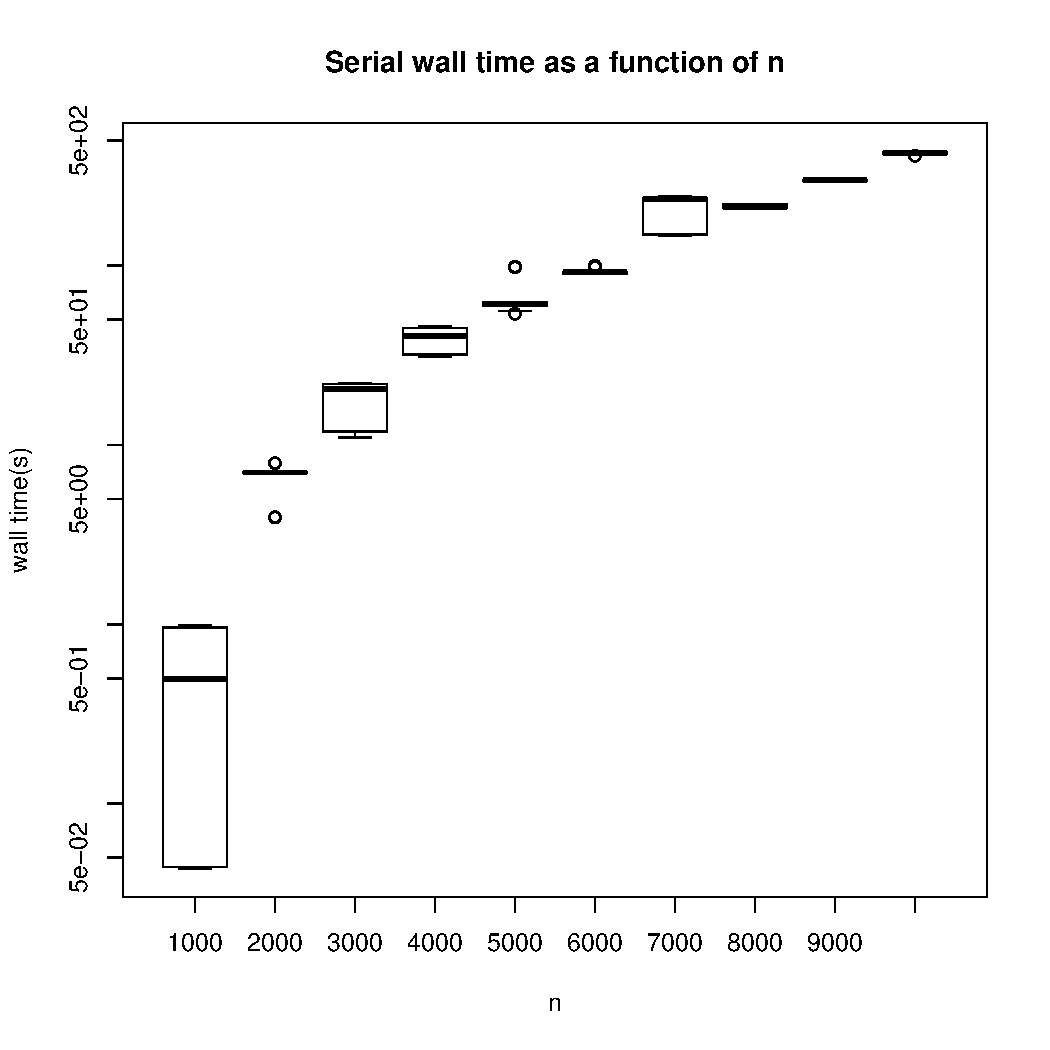
\includegraphics[width=12cm]{../analysis/serial_walltime_mkl.pdf}
  \end{center}
  \caption{Sequential implementation wall time as a function of problem size run on a single core.}
  \label{serial_walltime}
\end{figure}

\subsection{Parallel implementation wall time}
\begin{figure}[H]
  \begin{center}
    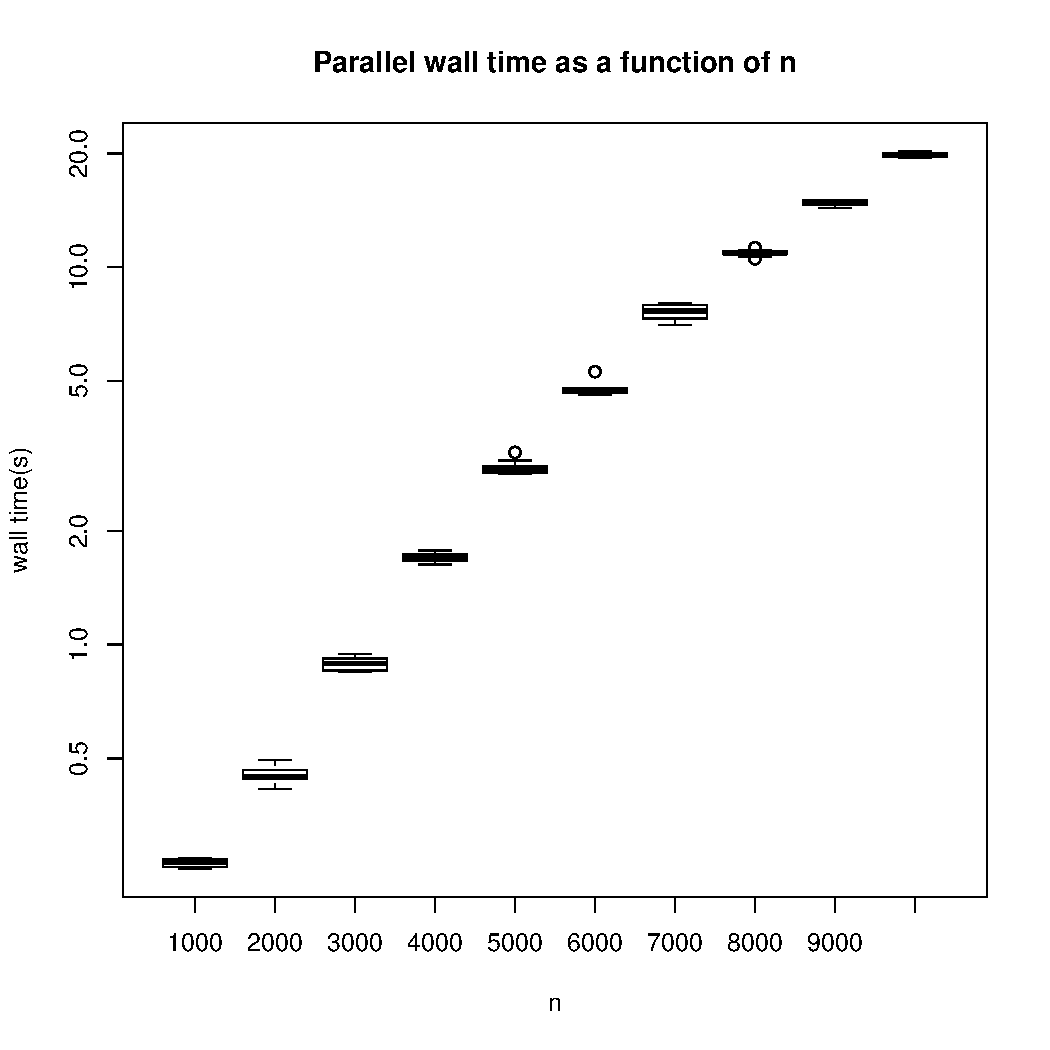
\includegraphics[width=12cm]{../analysis/parallel_problem_size_mkl.pdf}
  \end{center}
  \caption{Parallel implementation wall time as a function of problem size. Run on 5 nodes each with 5 MPI processes and 10 cores.}
  \label{parallel_walltime1}
\end{figure}

\begin{figure}[H]
  \begin{center}
    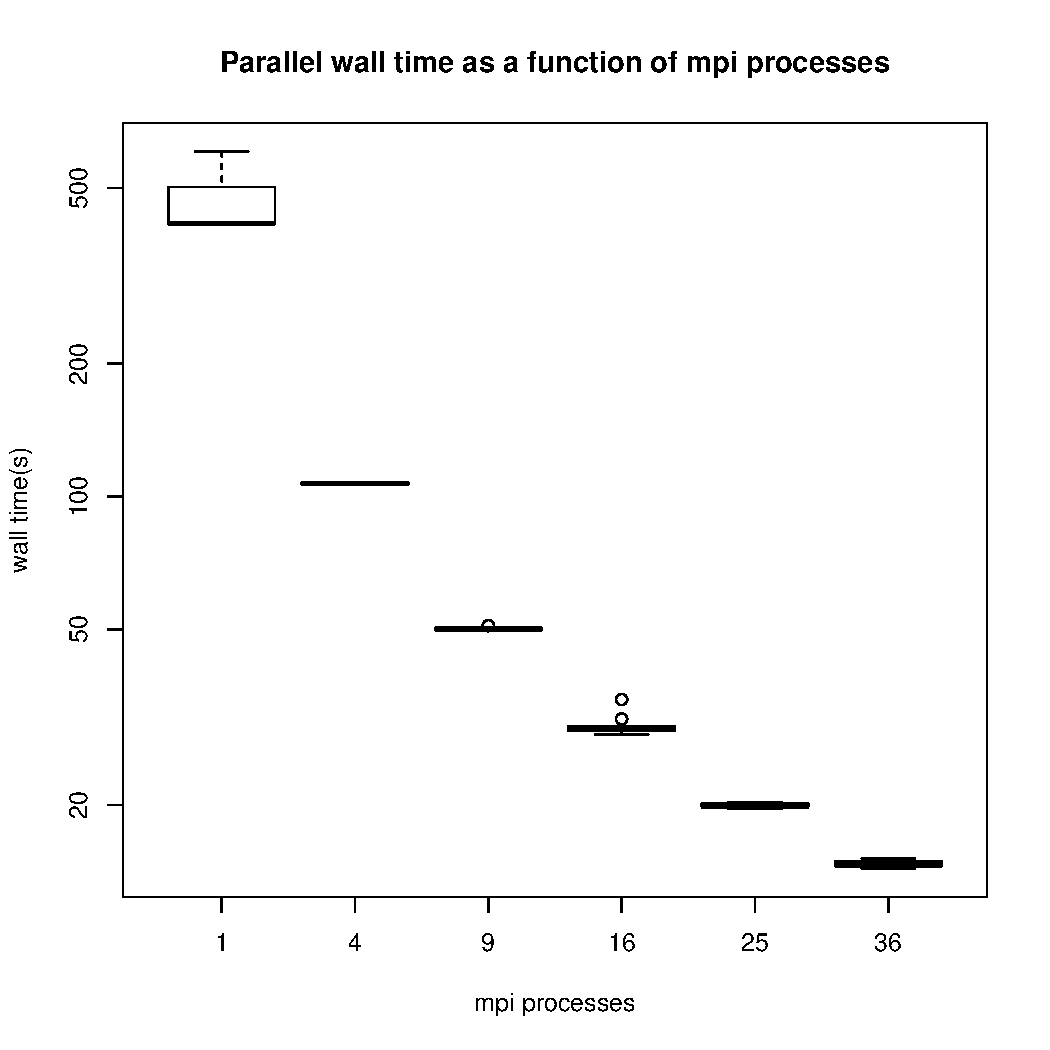
\includegraphics[width=12cm]{../analysis/mpi_nodes_walltime_mkl.pdf}
  \end{center}
  \caption{Parallel implementation wall time on a constant size problem, $n=10000$, as a function of mpi processes. For each mpi process there where two cores.}
  \label{parallel_walltime2}
\end{figure}

\subsection{Speedup}
\begin{figure}[H]
  \begin{center}
    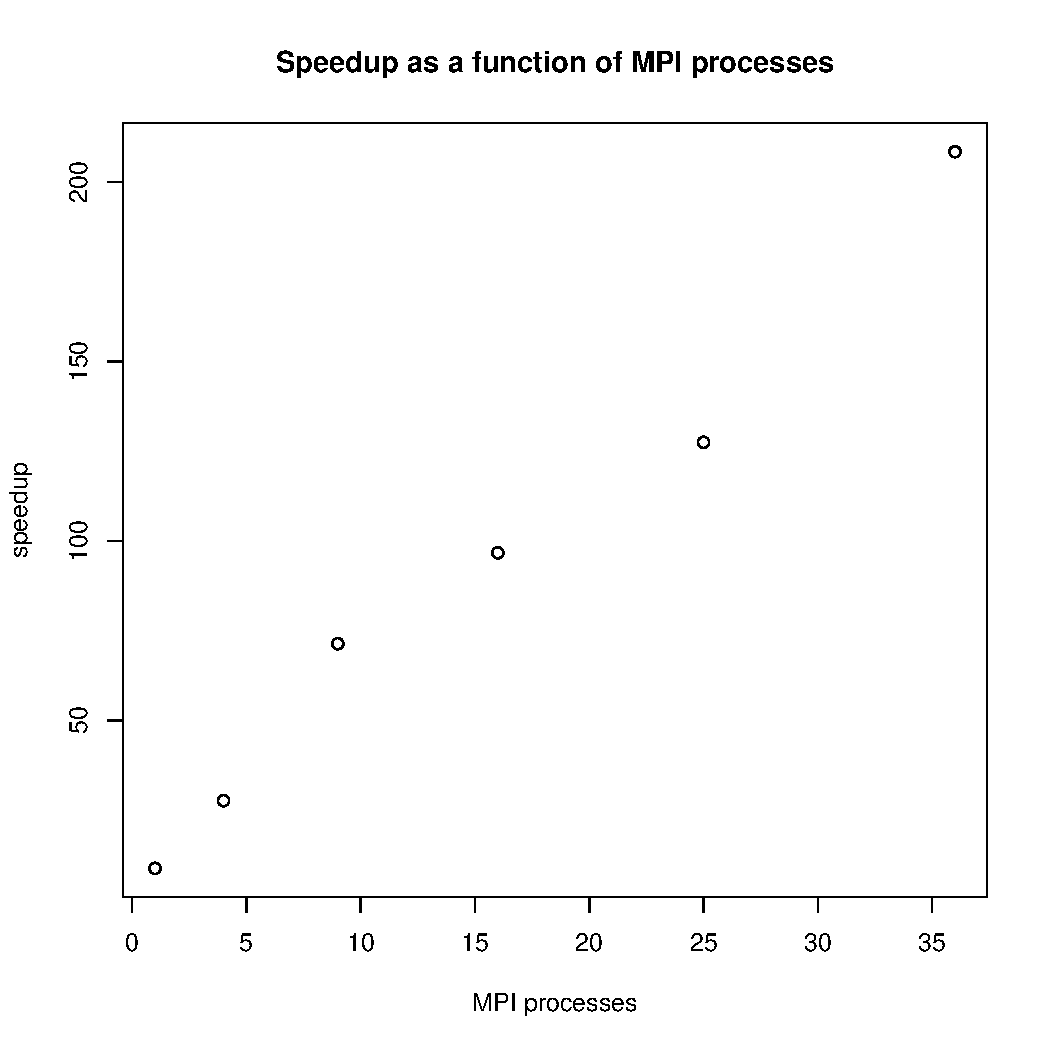
\includegraphics[width=12cm]{../analysis/mpi_nodes_speedup.pdf}
  \end{center}
  \caption{Speedup of program as a function of MPI processes when running on a constant problem size $n=10000$. For each MPI process there where two cores allocated to let OpenMP parallelize on the second core.}
  \label{mpi_nodes_speedup}
\end{figure}

\begin{figure}[H]
  \begin{center}
    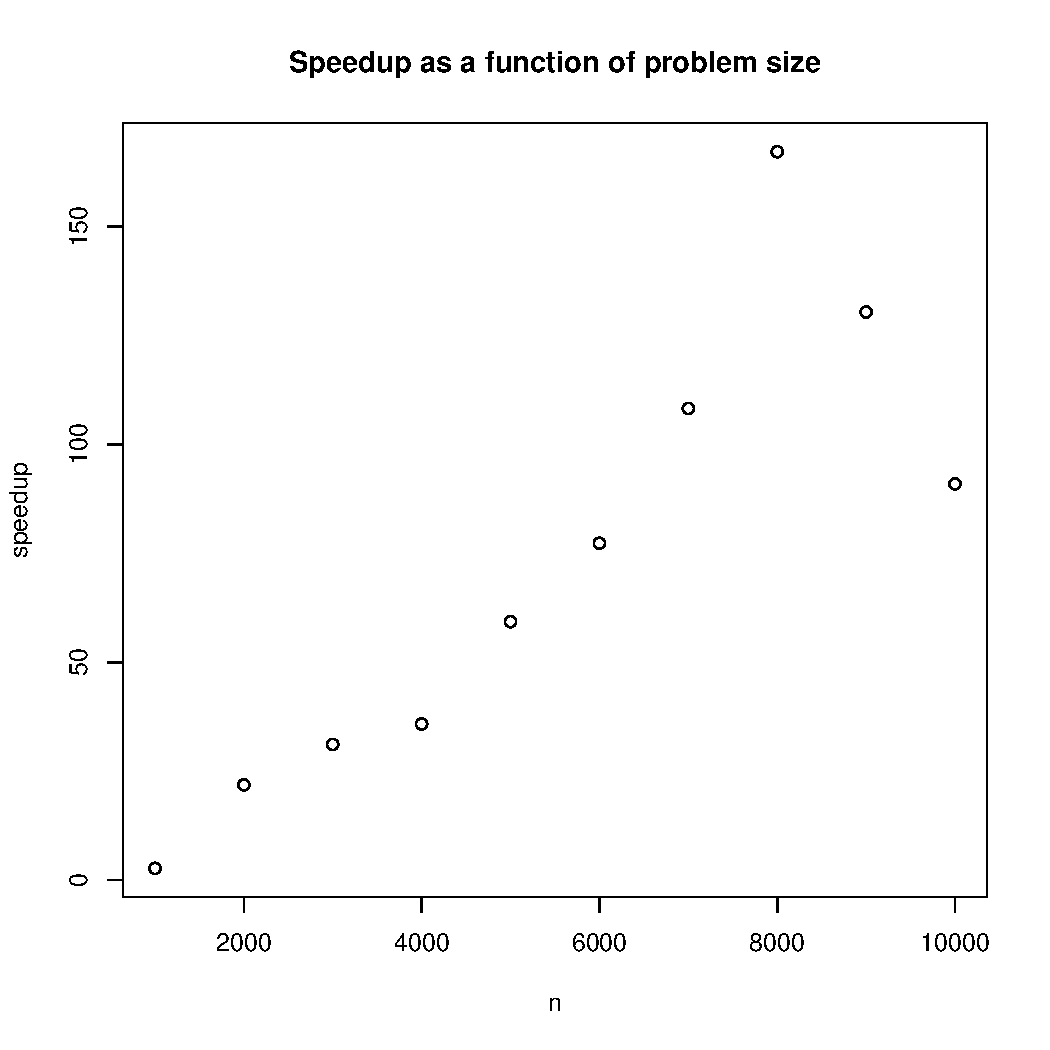
\includegraphics[width=12cm]{../analysis/problem_size_speedup.pdf}
  \end{center}
  \caption{Speedup of program as a function of problem size when running on a constant number of nodes, 5, MPI processes, 25, and cores, 50.}
  \label{problem_size_speedup}
\end{figure}

\section{Discussion}
The speedup observed in \ref{mpi_nodes_speedup}, \ref{problem_size_speedup}
will now be explained.
\subparagraph{Speedup as a function of problem size}
Even though the data is noisy there seems to be a quite constant
speedup of 15-20 times running on 
To explain the speedup of around 160 the following factors has
to be taken into consideration.

5 nodes where used. Each node had
5 mpi processes and 10 cores available. The remaining 5 cores on each
node would be saturated by the parallelism from the Intel MKL library.
All in all this adds up to 50 cores.

%Secondly, the sequential implementation did not use any hardware dependent
%optimizations. Most importantly the code was not vectorized. The parallel
%implementation used MKL which for dgemm uses AVX2 instructions to do
%4 double precision floating point operations at the same time. Because of
%this 2 to 4 times the speedup can be claimed to come from vectorization.

Secondly and most importantly. The sequential implementation runs on one core. This
gives it access to only that cores cache. Taking a closer look at the data sheet
for the E5-2670\cite{intel-datasheet} we observe that the cache hierarchy is
the following:
\begin{enumerate}
		\item L1 32kB instruction and 32kB data cache for each core
		\item L2 256kB shared instruction data cache for each core
		\item L3 20MB shared instruction data cache shared amongst all cores on the socket
\end{enumerate}
From a small calculation we see that for storing 3 1000x1000 matrices of doubles we need
\[
3 \times 1000^2 \frac{64}{8} = 3 \times 7.68 \text{Mb} = 22.89 \text{Mb}
\]
of memory.
Thus even the smallest problem, $n=1000$ will fill all the cache layers from L1 to L3.
For bigger problem this memory requirement increase on the order of $O(n^2)$.
When the cache is saturated the core will frequently have to go to RAM to get new parts of the problem. This memory
access is several orders of magnitude slower that accessing the cache and the program sees a big
slowdown because of it.

%Adding all these factors together, 50 cores, 2 to 4 times vectorization and at least 5 to 10 times slower memory access
Adding all these factors together, 50 cores and a conservative 2 to 5 times slower memory access
gives numbers close to
\[
%50 \times 2 \times 5 = 500 < \text{speedup} < 50 \times 4 \times 10 = 2000.
50 \times 2 = 100 < \text{speedup} < 50 \times 5 = 250.
\]
This means that without taking into account the synchronization overhead
%the parallel algorithm could see between 500 and 2000 times speedup in the given example.
the parallel algorithm could see between 100 and 250 times speedup in the given example.
The reason we are seeing about 20 is because
of all the synchronization introduced in the distributed algorithm.

\subparagraph{Speedup as a function of MPI processes}
The same considerations apply to the speedup as a function of MPI processes.
To explain the speedup of 200 you have to take into account that for each MPI
process there where 2 cores allocated. This means we where using 64 cores.
\[
%64 \times 2 \times 5 = 640 < \text{speedup} < 64 \times 4 \times 10 = 2560.
64 \times 2 = 128 < \text{speedup} < 64 \times 5 = 320.
\]
There is also here a considerable loss of speed because of synchronization.
Nevertheless the speedup seem very linear following the formula
\[
\text{speedup} = p\frac{3}{7}.
\]
If you double the number of cores you get a bit more than 40\%
speed increase.
%Nevertheless the speedup results are much better than expected.

\subsection{Feature suggestions and research questions}
The only big unanswered question is why a high level of SMP parallelism did not give better
results than distributed memory parallelism. The highly hardware,
library and compiler dependent nature of this problem makes it hard
to debug on QUTs HPC cluster because of limited profiling possibilities
etc. in a distributed MPI environment. Also the fact that you never are
logged in to the cluster nodes itself where your program is running makes
the whole debugging a lot harder. The authors theory is that the less L3
cache available for the versions running with higher SMP parallelizm ratio
is considerably slowing down the application.

\section{Conclusion}
The author considers the project a success both from a learning perspective and
the actual results. The author learnt a whole array of new technologies that
will be usefull in future work. The ability to use a real HPC facility for the
experiments definitly helped motivate the work. Learning industry
standard technologies as MPI, OpenMP and BLAS together with new mathematical
analytical skills, good engineering practice for numerical codes etc. was
very interesting. There is definitly possibilities for making a faster Poisson
solver by eg. using FFT algorithms, but this was not seen as the goal of
this report. The objective of making a general, fast and massively scalable
Poisson solver was achieved. Acknowledgements to QUT HPC staff for being
very helpfull with integration of the software into their platform.

\section{Appendix: Developed code}
All the code developed for this project is open sourced and available
in a version controled repository on the authors GitHub page \cite{github}.
The code run on the QUT HPC cluster is available under the summa folder. The \LaTeX source of this
report is available under the folder \verb+report+. All the timing data together with the R-script used
for analysis of this is available under the folder \verb+analysis+. There is also a working implementation of
matrix multiply written in the accelerate domain specific language in Haskell under the \verb+diagtest/diag-haskell+
folder. The \verb+doc+ folder contains reference documentation and papers used during the creation of this report.
\begin{em}To run a desktop version of the application run on the HPC cluster follow the \verb+README+ in the \verb+summa+ folder.\end{em}

\section{Appendix: Derivation of solution method}
\label{sec:math_der}
Poisson's equation is given as
\[
-\Delta u = f
\]
where $\Delta = \nabla^2$ is the Laplace operator, u and f are real or complex valued functions in a
euclidean space. The equation is often written as
\[
-\nabla^2 u = f.
\]
In two dimensions the equation can be written as
\[
-\left( \dd{}{x} + \dd{}{y}\right) u(x,y) = f(x,y).
\]

This equation is continuous and to work with it in the computer some discretized approximation has
to be made. This equation is continuous and to work with it in the computer some discretized approximation has to be made. A finite difference approximation was chosen as it presents us with a
problem that have several solution strategies that illustrates well the important properties to
consider when designing parallel numerical algorithms.

After a FDM discretization we are left with a 2D regular grid. Each node in this grid represents
a point for which we compute an approximation to our functions $u(x,y)$ and $f(x,y)$.
Using a central difference approximation to the partial derivatives in each direction leaves us
with the following equation
\[
-\frac{u_{i+1,j}-2u_{i,j}+u_{i-1,j}}{h^2} - \frac{u_{i,j+1}-2u_{i,j}+u_{i,j-1}}{h^2} = f_{i,j}, 1\leq i,j \leq n-1.
\]

The goal is to express this 2D equation as a linear system of equations which we then can solve with
different techniques using the computer.

Let
\begin{equation}
       U = \begin{bmatrix}
               u_{1,1} & \dots & u_{1,n} \\
               \vdots  &       & \vdots \\
               u_{n,1} & \dots & u_{n,n}
       \end{bmatrix}
\end{equation}
be the discretized version of $u$.

Let 
\begin{equation}
       T = \begin{bmatrix}
               2 & -1 & & & \\
               -1 & 2 & -1 & & \\
               & \ddots & \ddots & \ddots &\\
               & & -1 & 2 & -1\\
               & & & -1 & 2 \\
       \end{bmatrix}
\end{equation}
be the discrete partial double derivative operator.
Then,
\begin{align*}
       (TU)_{i,j} &= 2u_{i,j} - u_{i+1,j}, &i=1,\\
       (TU)_{i,j} &= 2u_{i,j} - u_{i+1,j} - u_{i-1,j}, &2 \leq i \leq n-2,\\
       (TU)_{i,j} &= 2u_{i,j} - u_{i-1,j}, &i=n-1.\\
\end{align*}
and thus,
\[
\frac{1}{h^2}(TU)_{i,j} \approx - \left( \dd{u}{x} \right)_{i,j}.
\]
By the same argument
\[
\frac{1}{h^2}(UT)_{i,j} \approx - \left(\dd{u}{y}\right)_{i,j}.
\]

Our finite difference scheme can thus be written as
\[
\frac{1}{h^2}(TU + UT)_{i,j} = f_{i,j}, \quad 1\leq i,j \leq n-1.
\]
Or
\[
\label{linsys}
TU + UT = G
\]
where
\begin{equation}
G = h^2 \begin{bmatrix}
               f_{1,1} & \dots & f_{1,n} \\
               \vdots  &       & \vdots \\
               f_{n,1} & \dots & f_{n,n}
       \end{bmatrix}
\end{equation}.

The $T$ matrix may be diagonalized
\[
T = Q \Lambda Q^\top
\]
where $\Lambda$ is a diagonal matrix and $Q Q^\top=I$, the identity matrix.
When we insert this expression for $T$ in \eqref{linsys} we get
\[
Q \Lambda Q^\top U + U Q \Lambda Q^\top = G.
\]
Multiplying from right with $Q$ and left with $Q^\top$ gives
\begin{align*}
&(Q^\top Q) \Lambda Q^\top U Q + Q^\top U Q \Lambda (Q^\top Q)\\
&= \Lambda Q^\top U Q + Q^\top U Q \Lambda = Q^\top G Q.
\end{align*}


\begin{thebibliography}{9}

\bibitem{github}
  \url{https://github.com/molysgaard/poisson}

\bibitem{summa}
  Robert A. van de Geijn and Jerrell Watts (1997)
  \emph{SUMMA: Scalable Universal Matrix Multiplication Algorithm}
  \url{http://www.netlib.org/lapack/lawnspdf/lawn96.pdf}
 
\bibitem{mkl}
  \url{http://software.intel.com/en-us/intel-mkl}

\bibitem{r-project}
  \url{http://www.r-project.org/}

\bibitem{haskell}
  \url{http://haskell.org}

\bibitem{accelerate}
  \url{http://hackage.haskell.org/package/accelerate}

\bibitem{blas}
  \url{http://www.netlib.org/blas/}

\bibitem{lapack}
  \url{http://www.netlib.org/lapack/}

\bibitem{intel-datasheet}
  \url{https://www-ssl.intel.com/content/dam/www/public/us/en/documents/datasheets/xeon-e5-v2-datasheet-vol-1.pdf}

\bibitem{boxplot}
  \url{http://en.wikipedia.org/wiki/Box_plot}

\end{thebibliography}

\end{document}
